%%%%%%%%%%%%%%%%%%%%%%%%%%%%%%%%%%%%%%%%%%%%%%%%%%%%%%%%%%%%%
%% HEADER
%% EDIT THIS FILE IN A BETTER APPLICATION THAN RSTUDIO
%%%%%%%%%%%%%%%%%%%%%%%%%%%%%%%%%%%%%%%%%%%%%%%%%%%%%%%%%%%%%
\documentclass[letterpaper,twoside,10pt]{article}
% Duplex: oneside / twoside

%% Language %%%%%%%%%%%%%%%%%%%%%%%%%%%%%%%%%%%%%%%%%%%%%%%%%
\usepackage[USenglish]{babel} %francais, polish, spanish, ...
\usepackage[T1]{fontenc}
\usepackage[ansinew]{inputenc}
\usepackage{lmodern} %Type1-font for non-english texts and characters

\usepackage{tabularx} %For setting table widths
\usepackage{float}
%\setcounter{topnumber}{2} %allow 2 floats (tables or figures) per top of page
%\setcounter{totalnumber}{3}
%\renewcommand{\floatpagefraction}{0.5} % % of pages that can have float at top
%\renewcommand{\topfraction}{0.85} % % of pages that can have float at top

%% Packages for Graphics & Figures %%%%%%%%%%%%%%%%%%%%%%%%%%
\usepackage{graphicx} %%For loading graphic files

%% Math Packages %%%%%%%%%%%%%%%%%%%%%%%%%%%%%%%%%%%%%%%%%%%%
%\usepackage{amsmath}
%\usepackage{amsthm}
%\usepackage{amsfonts}


%% Line Spacing %%%%%%%%%%%%%%%%%%%%%%%%%%%%%%%%%%%%%%%%%%%%%
%\usepackage{setspace}
%\singlespacing        %% 1-spacing (default)
%\onehalfspacing       %% 1,5-spacing
%\doublespacing        %% 2-spacing

%% Other Packages %%%%%%%%%%%%%%%%%%%%%%%%%%%%%%%%%%%%%%%%%%%
\usepackage[margin=1in]{geometry}

%%%%%%%%%%%%%%%%%%%%%%%%%%%%%%%%%%%%%%%%%%%%%%%%%%%%%%%%%%%%%
%% DOCUMENT
%%%%%%%%%%%%%%%%%%%%%%%%%%%%%%%%%%%%%%%%%%%%%%%%%%%%%%%%%%%%%
\begin{document}

\pagestyle{empty} %No headings for the first pages.

\title{Sample for Integrating R Output with Latex}
\author{Jim Marquardson}
%\date{} %%If commented, the current date is used.
\maketitle

\pagestyle{plain} %Now display headings: headings / fancy / ...

\section{Introduction}\label{Introduction}

This file was generated using R, RStudio, Miktex, Ghostscript, and make. Here is a citation \cite{IsaacNewton}.

\section{In Latex}\label{InLatex}

Use \textbackslash{}input\{petDancing\} to include an external tex file.

\begin{figure}[htb]
  \centering
		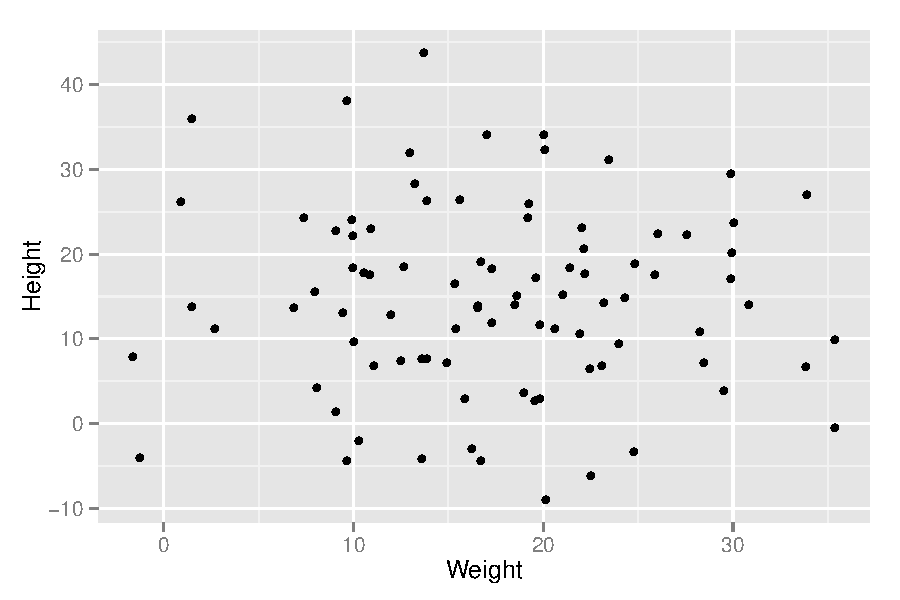
\includegraphics{../figures/scatter.pdf}
	\caption{Sample Scatter Plot}
	\label{fig:scatter}
\end{figure}

Figure ~\ref{fig:scatter} shows a scatterplot for animal weight and height. The table ~\ref{tab:petColor} shows the counts for pets and color. The p value is 3.14159
\unskip.

% latex table generated in R 2.15.2 by xtable 1.7-1 package
% Tue Mar 26 21:10:08 2013
\begin{table}[ht]
\centering
\begin{tabular}{|l|l|l|l|l|}
  \hline
 & Black & Brown & Yellow & Gray \\ 
  \hline
Dog &  15 &  20 &   7 &   0 \\ 
  Cat &   0 &   0 &  23 &  25 \\ 
   \hline
\end{tabular}
\caption{Pets and Color.\label{tab:petColor}} 
\end{table}


\section{References}\label{references}

%%%%%%%%%%%%%%%%%%%%%%%%%%%%%%%%%%%%%%%%%%%%%%%%%%%%%%%%%%%%%
%% BIBLIOGRAPHY AND OTHER LISTS
%%%%%%%%%%%%%%%%%%%%%%%%%%%%%%%%%%%%%%%%%%%%%%%%%%%%%%%%%%%%%

%% The Bibliography
%% ==> You need to run BibTeX for this (Project | Properties... | Uses BibTeX)
%\addcontentsline{toc}{chapter}{Bibliography} %'Bibliography' into toc
%\nocite{*} %Even non-cited BibTeX-Entries will be shown.
%\bibliographystyle{alpha} %Style of Bibliography: plain / apalike / amsalpha / ...
\bibliographystyle{plain}
\bibliography{bibliography} %You need a file 'bibliography.bib' for this.

\end{document}
